% !TEX root = ../Thesis.tex
\chapter{Background}

This section provides background explanations for key concepts as they relate to this thesis. The concepts covered are the sliding tile 
puzzle ($\ref{section:slidingtile}$, pattern databases \dots

\section{Sliding Tile Puzzle} \label{section:slidingtile}

The classic sliding tile puzzle (or 15-puzzle) is a two dimensional combination puzzle composed of 15 numbered tiles and one empty tile arranged in a 
four by four square. The position of the empty tile can be swapped with edge adjacent tiles. The goal of the puzzle is to reach a state where the 
numbered tiles are in row-wise ascending order starting from the top left and the empty tile is at a specified position (typically the top left).

\begin{figure}
\centering
\subfigure[Unsolved]{\label{fig:a}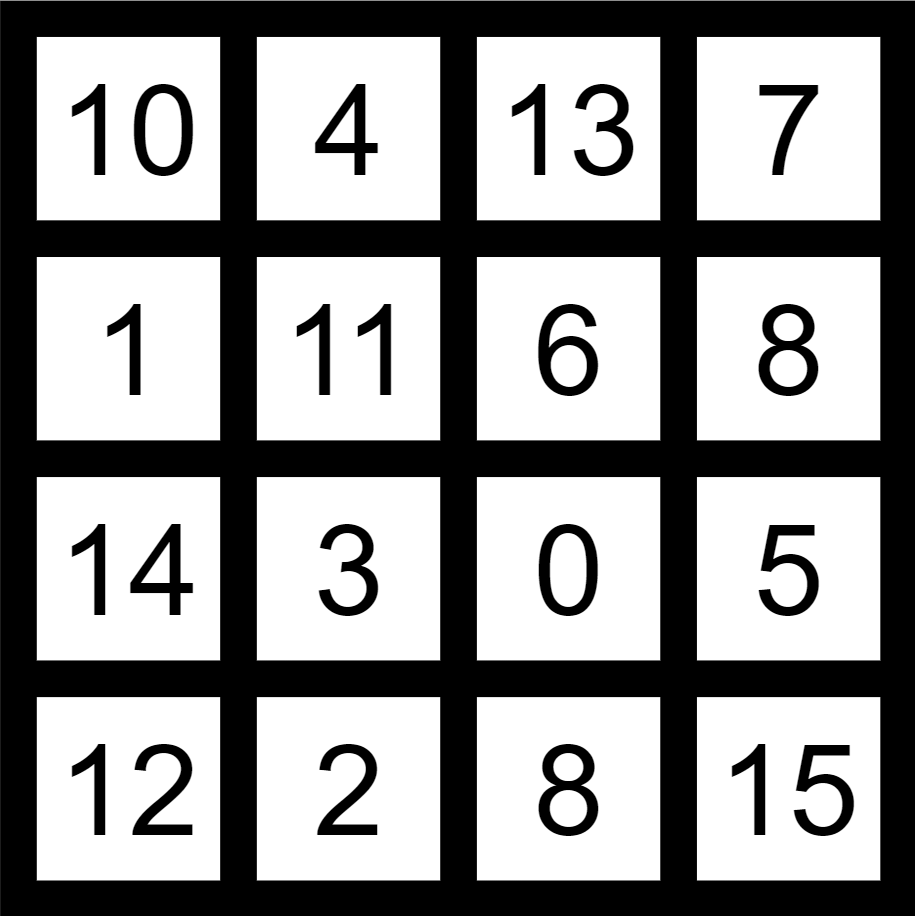
\includegraphics[width=60mm]{Figures/UnsolvedSlidingTilePuzzle.png}}
\subfigure[Solved]{\label{fig:b}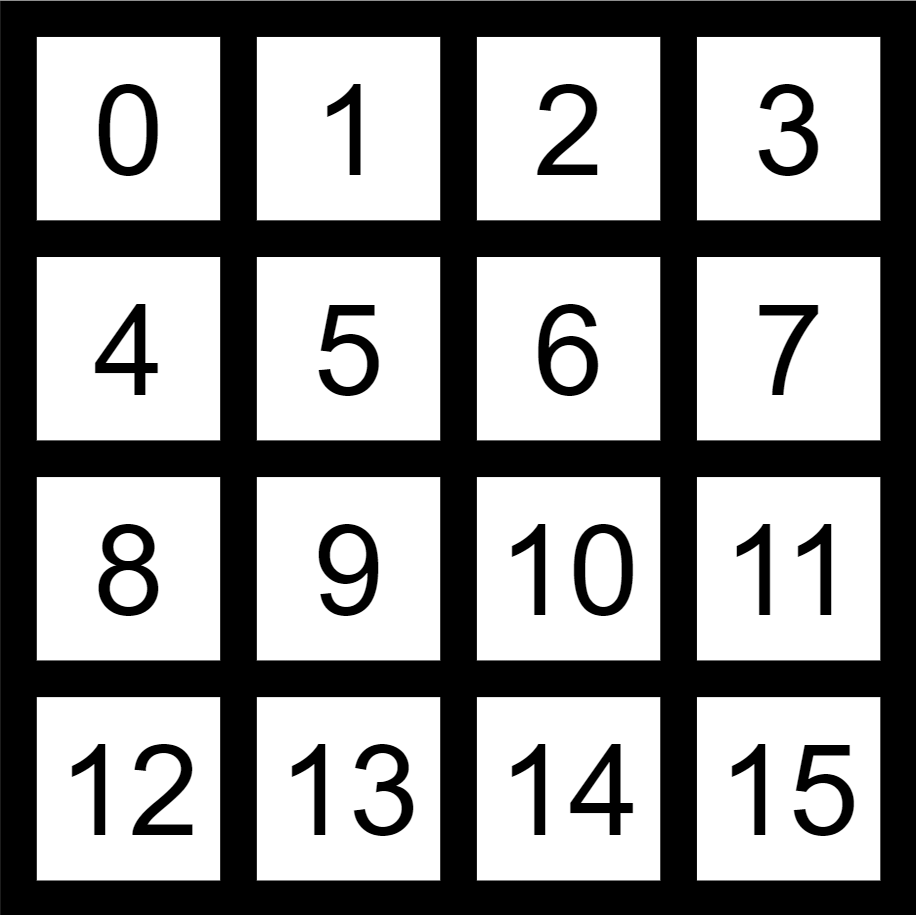
\includegraphics[width=60mm]{Figures/SolvedSlidingTilePuzzle.png}}
\caption{Examples of a solved \ref{fig:b} and unsolved \ref{fig:b} STP state}
\end{figure}

The number of theoretically possible starting states the puzzle can assume is 16!, of which half are unsolvable and the other half is solvable. In effect, the unsolvable states can never be reached from any of the solvable states, as long as only legal swap actions are taken, and vice versa. 

In memory we can represent each state of the puzzle with an array of length 16, where the value at index $i \in \{0, ..., 15\}$ is the number of the tile at the ith spot in the puzzle starting from the top left going row wise. Swapping the blank tile with an adjacent tile then simply requires swapping the two respective entries in the array.

\section{Pattern Databases} 

Pattern Databases (PDB) are among the most commonly used abstraction heuristics in search and planning \cite{helmert:pdb}. For the sliding tile puzzle, they were first introduced in 1996 by Culberson and Schaeffner \cite{culberson:pdb} \cite{culberson:swpdb}.

A \textbf{pattern} is a set of tiles that is also a subset of the set containing all 16 tiles. Each pattern must include the empty tile. We then consider an abstract state, where the numbers associated with all other tiles except those in the pattern are replaced with blank tiles. Note the difference between a blank tile and the empty tile, which is denoted with the number zero.
A \textbf{target pattern} is a pattern constructed from the goal state as described above.
A \textbf{pattern database} is a mapping for all possible permutations of a target pattern to a heuristic value, that corresponds to the number of moves (or distance) from the target pattern. It can be constructed by utilizing a breadth first search from the goal state.

The heuristic returned by the pattern database for an abstract state is a lower bound on the number of moves required for the full state of the puzzle. \cite{culberson:pdb}




A search using pattern databases involves the following steps. First, we do a depth first search \cite{sturtevant:sas}

For the sliding tile puzzle the common approach previously was to 

\section{Post-Hoc Optimization}

TODO

